%!TEX root = ../../report.tex
\section{Feature map for Monte Carlo localization}
For the Monte Carlo localization the features that is desired are static object like buildings, heavy machinery, etc. These share the property of not moving. The elements added for the localization should therefore be cells that have been very static. In the interpretation step each cell is classified as static or non-static. Cells that have been classified as static are given the maximum value, lethal, in the costmap. 
The parameters available for classification are:
\begin{itemize} 
\item Sum of occupied scores
\item Sum of free scores
\item Sum of exit events
\item Sum of entry events
\item Previous observation
\item \(\lambda_{exit}\) - estimated by exit events and occupied scores
\item \(\lambda_{entry}\) - estimated by entry events and free scores
\end{itemize}

We propose a simple classifier that bases its decisions on \(\lambda_{exit}\), the sum of occupied scores and the sum of free scores.  \(\lambda_{exit}\) is chosen because one of the primary requirements is that the probability of the cell to switch to free should be very low for static obstacles. The two sums are used to ensure that the cells has been more occupied than free. 
The classification rules was determined based on simulation as well as real world data. In figure \ref{fig:amcl_classifier} is shown the classification results as well as the ground truth. Figure \ref{fig:amcl_classifier:worst} shows a bad classifier that includes all the dynamic obstacles. The results from the chosen classifier are shown in figure \ref{fig:amcl_classifier:chosen}. In the result almost all of the dynamic obstacles are removed. It was not possible to adjust the limits to suppress the remaining dynamical obstacles without damaging the true walls. In the simulation the robot drove from the top-right corner to the bottom-left. This means that the amount of data from the two remaining corners are very limited. 

%% FIGURE - CLASSIFICATIONS
\begin{figure}[htbp]
	\label{fig:amcl_classifier}
	\begin{subfigure}{.5\textwidth}
		\centering
		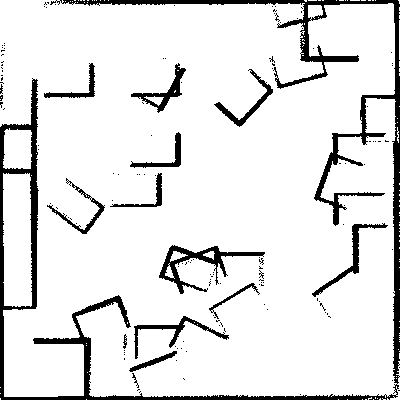
\includegraphics[width=1\linewidth]{chapters/cost_interpretation/figures/occ_above_0_classifier.png}
		\caption{Obstacles: \(\Sigma state_{occ} > \Sigma state_{free}\)}
		\label{fig:amcl_classifier:worst}
	\end{subfigure}
	\qquad
	\begin{subfigure}{.5\textwidth}
		\centering
		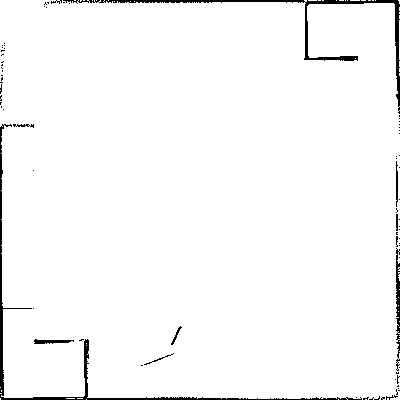
\includegraphics[width=1\linewidth]{chapters/cost_interpretation/figures/chosen_classifier.png}
		\caption{Obstacles: \(\Sigma state_{occ} > 2 \cdot \Sigma state_{free}\) and \(\lambda_{exit} < 0.15\) }
		\label{fig:amcl_classifier:chosen}
	\end{subfigure}\\[1ex]
	\begin{subfigure}{1\textwidth}
		\centering
		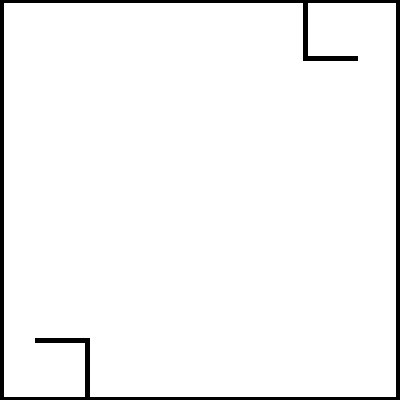
\includegraphics[width=.5\linewidth]{chapters/cost_interpretation/figures/dynamic_area_web.png}
		\caption{Ground truth map}
		\label{fig:amcl_classifier:groundtruth}
	\end{subfigure}
	
	\caption{Results of different classifier rules and the true map}
\end{figure}
